\documentclass[11pt,a4paper]{article}

% ------------------------------------------------------------------
% Packages
% ------------------------------------------------------------------
\usepackage[utf8]{inputenc}
\usepackage[T1]{fontenc}
\usepackage{lmodern}
\usepackage[margin=2.5cm]{geometry}
\usepackage{amsmath,amssymb}
\usepackage{graphicx}
\usepackage{float}          % lets us use [H] to keep figures/tables in place
\usepackage{booktabs}       % nicer table lines
\usepackage{multirow}       % one cell spanning several table rows
\usepackage{caption}
\usepackage{hyperref}
\hypersetup{colorlinks=true, linkcolor=blue, citecolor=blue, urlcolor=blue}

% Figures are in ../figures/ when compiling inside paper/,
% or in figures/ when the folder is uploaded next to main.tex (e.g. Overleaf).
\graphicspath{{../figures/}{figures/}}

\title{Overall Survival Prediction in Adult Myeloid Leukemia:\\
Kaplan--Meier, Cox Regression and Machine-Learning Survival Models}
\author{Bernard Frimpong\\
\small M.S. Applied Mathematics, University of Akron}
\date{Working draft --- Stage 2 (Kaplan--Meier and the metric), October 2026}

\begin{document}
\maketitle

\begin{abstract}
This report documents my work on the QRT $\times$ Institut Gustave Roussy data
challenge on Challenge Data (ENS Paris), whose goal is to rank adult patients with
myeloid leukemia by their risk of death, using clinical measurements, cytogenetic
reports and somatic gene mutations. Models are scored with the inverse probability
of censoring weighted (IPCW) concordance index truncated at seven years. The data
audit shows that the 1{,}193 test patients all come from a single clinical centre that
is absent from the 23 training centres, and that this centre's patients are clinically
sicker, so model validation will hold out whole centres. Kaplan--Meier analysis gives a
median overall survival of 3.15 years, with strong separation by bone-marrow blasts,
\textit{TP53} and \textit{SF3B1} mutations and monosomy~7 (log-rank $p<0.001$ for all).
The Kaplan--Meier estimator, a log-rank test and both concordance indices were computed
by hand and match standard software. Single variables reach an IPCW C-index of at most
0.616, which is the baseline that multivariable models must beat.
\end{abstract}

% ==================================================================
\section{Introduction}
% ==================================================================
Myeloid leukemias are blood cancers in which abnormal immature cells (blasts)
accumulate in the bone marrow. Estimating a patient's prognosis guides treatment:
low-risk patients may receive supportive care, while high-risk patients may be
prioritised for intensive treatment such as stem cell transplantation.

The outcome is \emph{overall survival} (OS): the time from diagnosis to death or to the
last follow-up. When a patient is still alive at the last follow-up, the true survival
time is unknown; we only know it is longer than the observed time. Such observations
are called \emph{right-censored}, and handling them correctly is the purpose of
survival analysis.

The project follows a staged plan:
Kaplan--Meier estimation and log-rank tests,
Cox proportional hazards regression,
and machine-learning survival models (gradient-boosted survival and random survival
forests), all compared under the challenge metric with honest cross-validation.
A similar crowdsourced effort, the DREAM 9 AML Outcome Prediction Challenge, also
scored survival models with a concordance index~\cite{noren2016}.

% ==================================================================
\section{Data}
% ==================================================================
The data come from 24 clinical centres and are split into the five files described in
Table~\ref{tab:files}. The \texttt{ID} column links the files.

\begin{table}[H]
\centering
\caption{The five challenge files.}
\label{tab:files}
\begin{tabular}{lrl}
\toprule
File & Rows & Content \\
\midrule
\texttt{clinical\_train.csv}  & 3{,}323  & one row per patient: centre, blood counts, karyotype \\
\texttt{clinical\_test.csv}   & 1{,}193  & same, for test patients \\
\texttt{molecular\_train.csv} & 10{,}935 & one row per somatic mutation \\
\texttt{molecular\_test.csv}  & 3{,}089  & same, for test patients \\
\texttt{target\_train.csv}    & 3{,}323  & \texttt{OS\_YEARS}, \texttt{OS\_STATUS} \\
\bottomrule
\end{tabular}
\end{table}

\paragraph{Clinical variables.}
\texttt{BM\_BLAST} (bone-marrow blasts, \%), \texttt{WBC} (white blood cells, G/L),
\texttt{ANC} (absolute neutrophil count, G/L), \texttt{MONOCYTES} (G/L),
\texttt{HB} (haemoglobin, g/dL), \texttt{PLT} (platelets, G/L) and
\texttt{CYTOGENETICS}, a free-text karyotype written in ISCN notation
(for example \texttt{46,xy} for a normal male karyotype).

\paragraph{Molecular variables.}
Each row is one somatic mutation, with its chromosomal position, reference and
alternate bases, the gene, the protein change, the broad effect, the variant allele
fraction (\texttt{VAF}, the share of sequencing reads carrying the mutation) and, not
mentioned in the challenge description, the sequencing read depth (\texttt{DEPTH}).

% ==================================================================
\section{The evaluation metric}
\label{sec:metric}
% ==================================================================
For each patient $i$ we observe a time $T_i$ (\texttt{OS\_YEARS}), an event indicator
$\Delta_i$ (1 = death, 0 = censored), and the model gives a risk score $\eta_i$.

\paragraph{Harrell's C-index.}
A pair of patients $(i,j)$ is \emph{comparable} when we know who died first, that is,
when $T_i < T_j$ and patient $i$ died ($\Delta_i = 1$). The pair is \emph{concordant}
when the model agrees, $\eta_i > \eta_j$. Harrell's C-index~\cite{harrell1982} is
\begin{equation}
C = \frac{\text{number of concordant comparable pairs}}{\text{number of comparable pairs}}.
\label{eq:harrell}
\end{equation}
A value of $0.5$ corresponds to random guessing and $1$ to a perfect ranking. Pairs
with equal risk scores count as one half.

\paragraph{IPCW C-index (Uno's C).}
Patients who die late are less likely to be observed dying, because many patients are
censored before then. Harrell's C therefore over-represents early deaths. Uno
\textit{et al.}~\cite{uno2011} correct this by weighting each comparable pair by
$1/\hat G(T_i)^2$, where $\hat G(t)$ is the Kaplan--Meier estimate of the probability
of \emph{not yet being censored} at time $t$. With the truncation horizon $\tau = 7$
years used by the challenge,
\begin{equation}
C_\tau = \frac{\displaystyle\sum_{i}\sum_{j} \Delta_i\,\hat G(T_i)^{-2}\,
\mathbf{1}(T_i < T_j,\ T_i < \tau)\,\mathbf{1}(\eta_i > \eta_j)}
{\displaystyle\sum_{i}\sum_{j} \Delta_i\,\hat G(T_i)^{-2}\,
\mathbf{1}(T_i < T_j,\ T_i < \tau)}.
\label{eq:uno}
\end{equation}
In plain language: a death at a time when few patients remain uncensored is rare to
observe, so it counts more. Only the ordering of the scores $\eta_i$ matters. The
challenge computes $C_\tau$ with \texttt{scikit-survival}~\cite{polsterl2020}.

% ==================================================================
\section{Data audit (Stage 1)}
% ==================================================================

\subsection{Linking and outcome}
All IDs are unique, every mutation row belongs to a known patient, and no patient
appears in both training and test sets. However, 150 training patients have no
recorded outcome and are excluded from modelling. Table~\ref{tab:outcome} summarises
the remaining outcomes and Figure~\ref{fig:followup} shows the observed times.

\begin{table}[H]
\centering
\caption{Outcome of the training patients.}
\label{tab:outcome}
\begin{tabular}{lr}
\toprule
Quantity & Value \\
\midrule
Training patients                           & 3{,}323 \\
Without outcome (excluded)                  & 150 \\
With outcome                                & 3{,}173 \\
Deaths ($\Delta = 1$)                       & 1{,}600 (50.4\%) \\
Censored ($\Delta = 0$)                     & 1{,}573 (49.6\%) \\
Median observed time (years)                & 1.65 \\
Maximum observed time (years)               & 22.04 \\
Observed time exactly 0 (all censored)      & 53 \\
Observed beyond the 7-year horizon          & 172 \\
\bottomrule
\end{tabular}
\end{table}

\begin{figure}[H]
\centering
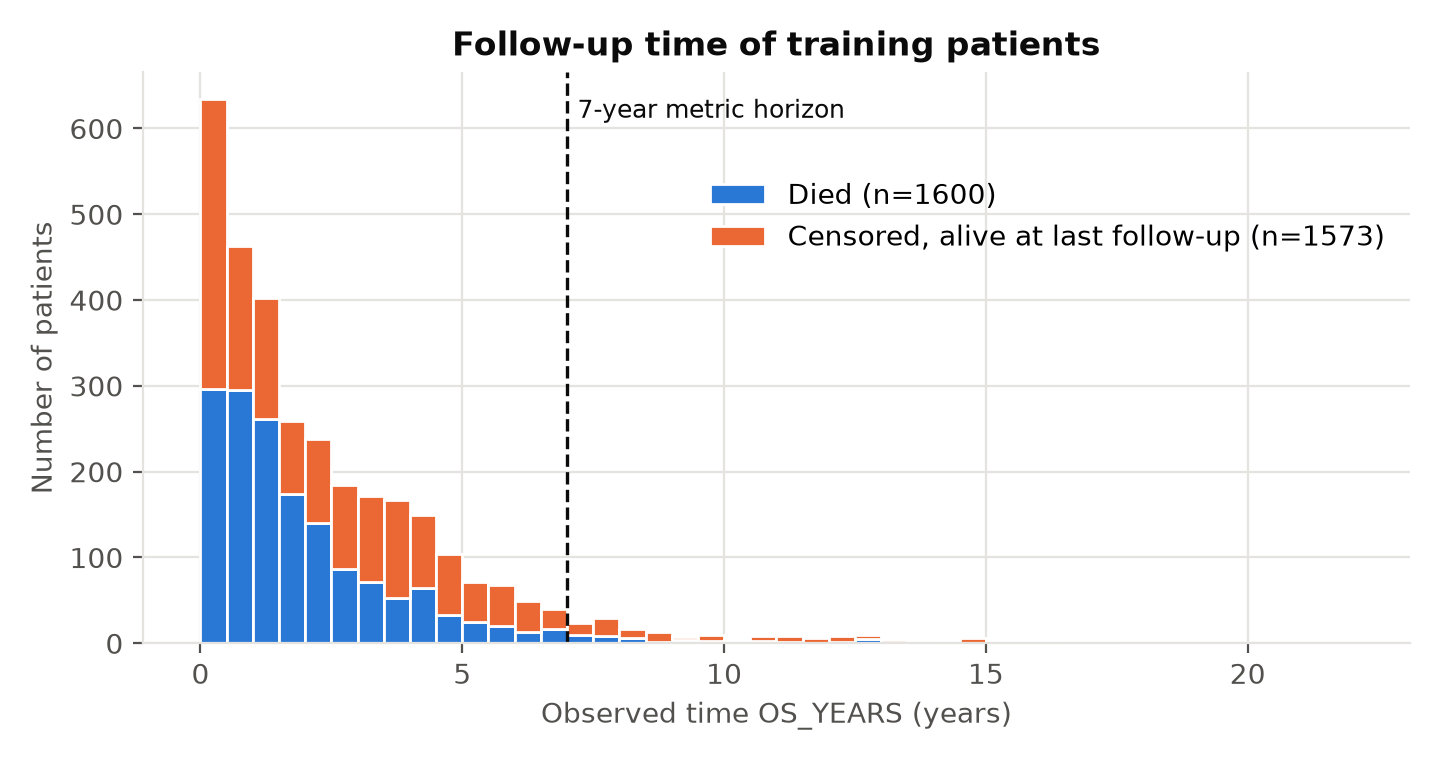
\includegraphics[width=0.9\textwidth]{fig04_followup.png}
\caption{Observed time of the 3{,}173 training patients with an outcome, split into
deaths and censored patients. The dashed line marks the 7-year horizon of the metric.}
\label{fig:followup}
\end{figure}

About half the patients are censored, so simply discarding them or treating their
observed time as a death time would badly bias any model. Most deaths occur within
the first two years, and only 172 patients are followed beyond seven years, which
justifies the truncation of the metric.

\subsection{Clinical centres: the test set is a new hospital}
The 3{,}323 training patients come from 23 centres, while all 1{,}193 test patients
come from one centre, \texttt{KYW}, that does not appear in training
(Figure~\ref{fig:centers}). Death rates also vary widely between training centres,
from 11\% (\texttt{ROM}) to 92\% (\texttt{MUV}), reflecting different patient
populations and follow-up lengths.

\begin{figure}[H]
\centering
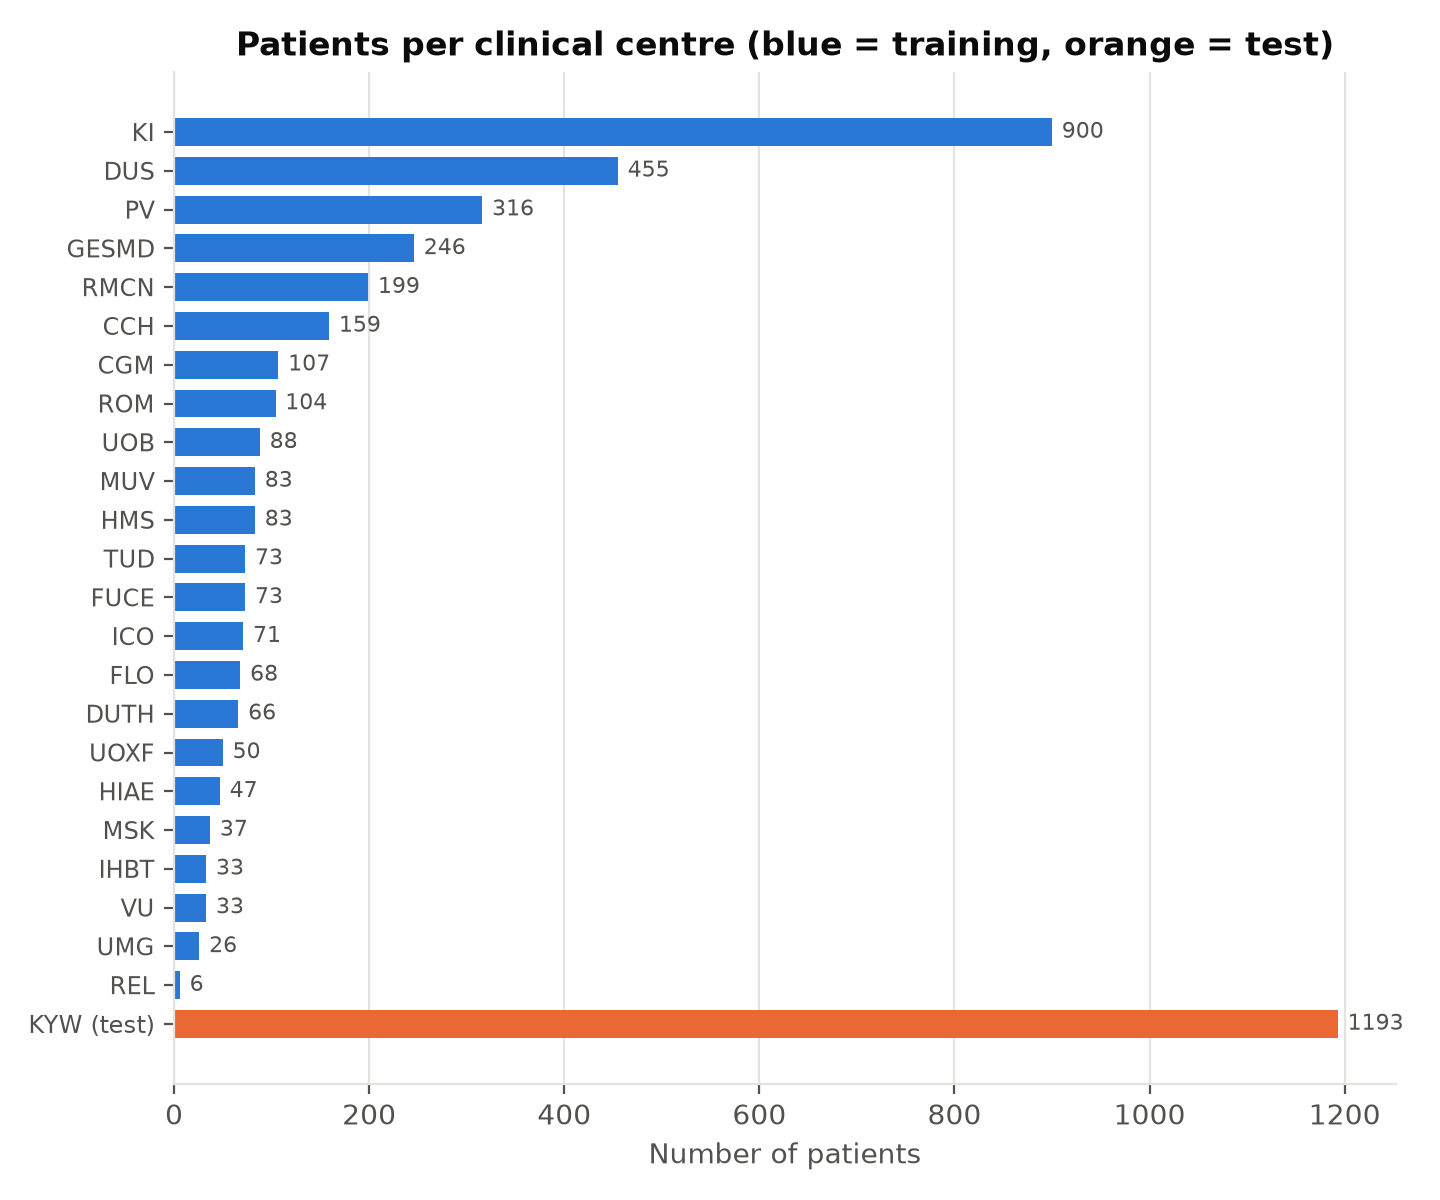
\includegraphics[width=0.8\textwidth]{fig03_centers.png}
\caption{Number of patients per clinical centre. The test centre \texttt{KYW} (orange)
contributes no training patients.}
\label{fig:centers}
\end{figure}

This has a direct consequence for validation. A random $K$-fold split mixes patients
from the same centre into training and validation folds, so the model is always
validated on centres it has already seen. The real task is to predict for an
\emph{unseen} centre. Cross-validation will therefore be grouped by centre, and the
\texttt{CENTER} variable cannot be used as a predictor.

\subsection{Clinical variables: training versus test}
Table~\ref{tab:clinical} and Figures~\ref{fig:missing} and~\ref{fig:dist} compare the
clinical variables in the two sets.

\begin{table}[H]
\centering
\caption{Missing values and medians of the clinical variables.}
\label{tab:clinical}
\begin{tabular}{lrrrr}
\toprule
 & \multicolumn{2}{c}{Missing (\%)} & \multicolumn{2}{c}{Median} \\
\cmidrule(lr){2-3}\cmidrule(lr){4-5}
Variable & Train & Test & Train & Test \\
\midrule
\texttt{BM\_BLAST} (\%)     & 3.3  & 9.6  & 3.00   & 6.00 \\
\texttt{WBC} (G/L)          & 8.2  & 9.4  & 4.10   & 2.90 \\
\texttt{ANC} (G/L)          & 5.8  & 11.8 & 2.00   & 1.30 \\
\texttt{MONOCYTES} (G/L)    & 18.1 & 74.0 & 0.37   & 0.20 \\
\texttt{HB} (g/dL)          & 3.3  & 9.3  & 9.70   & 8.40 \\
\texttt{PLT} (G/L)          & 3.7  & 9.6  & 123.00 & 74.00 \\
\texttt{CYTOGENETICS}       & 11.6 & 9.7  & --     & -- \\
\bottomrule
\end{tabular}
\end{table}

\begin{figure}[H]
\centering
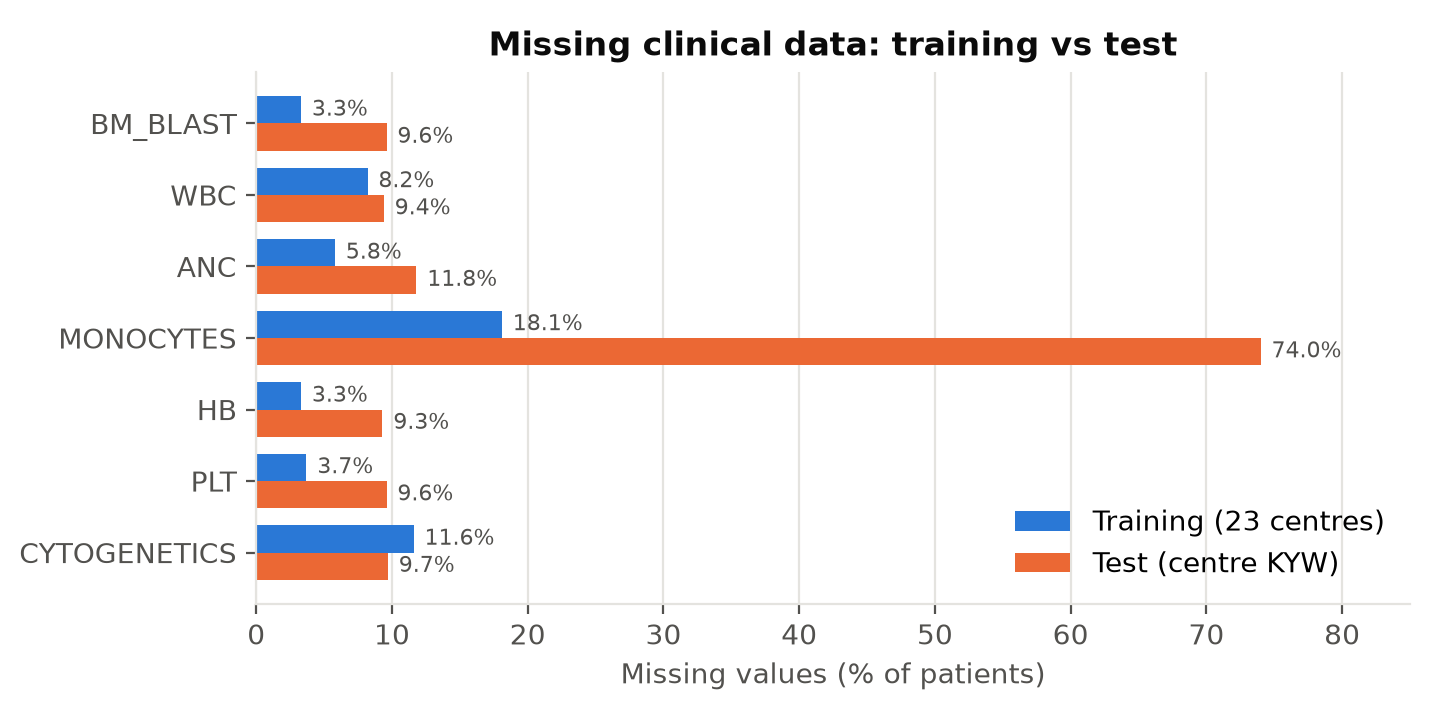
\includegraphics[width=0.85\textwidth]{fig01_missing_values.png}
\caption{Percentage of missing values in each clinical variable.}
\label{fig:missing}
\end{figure}

\begin{figure}[H]
\centering
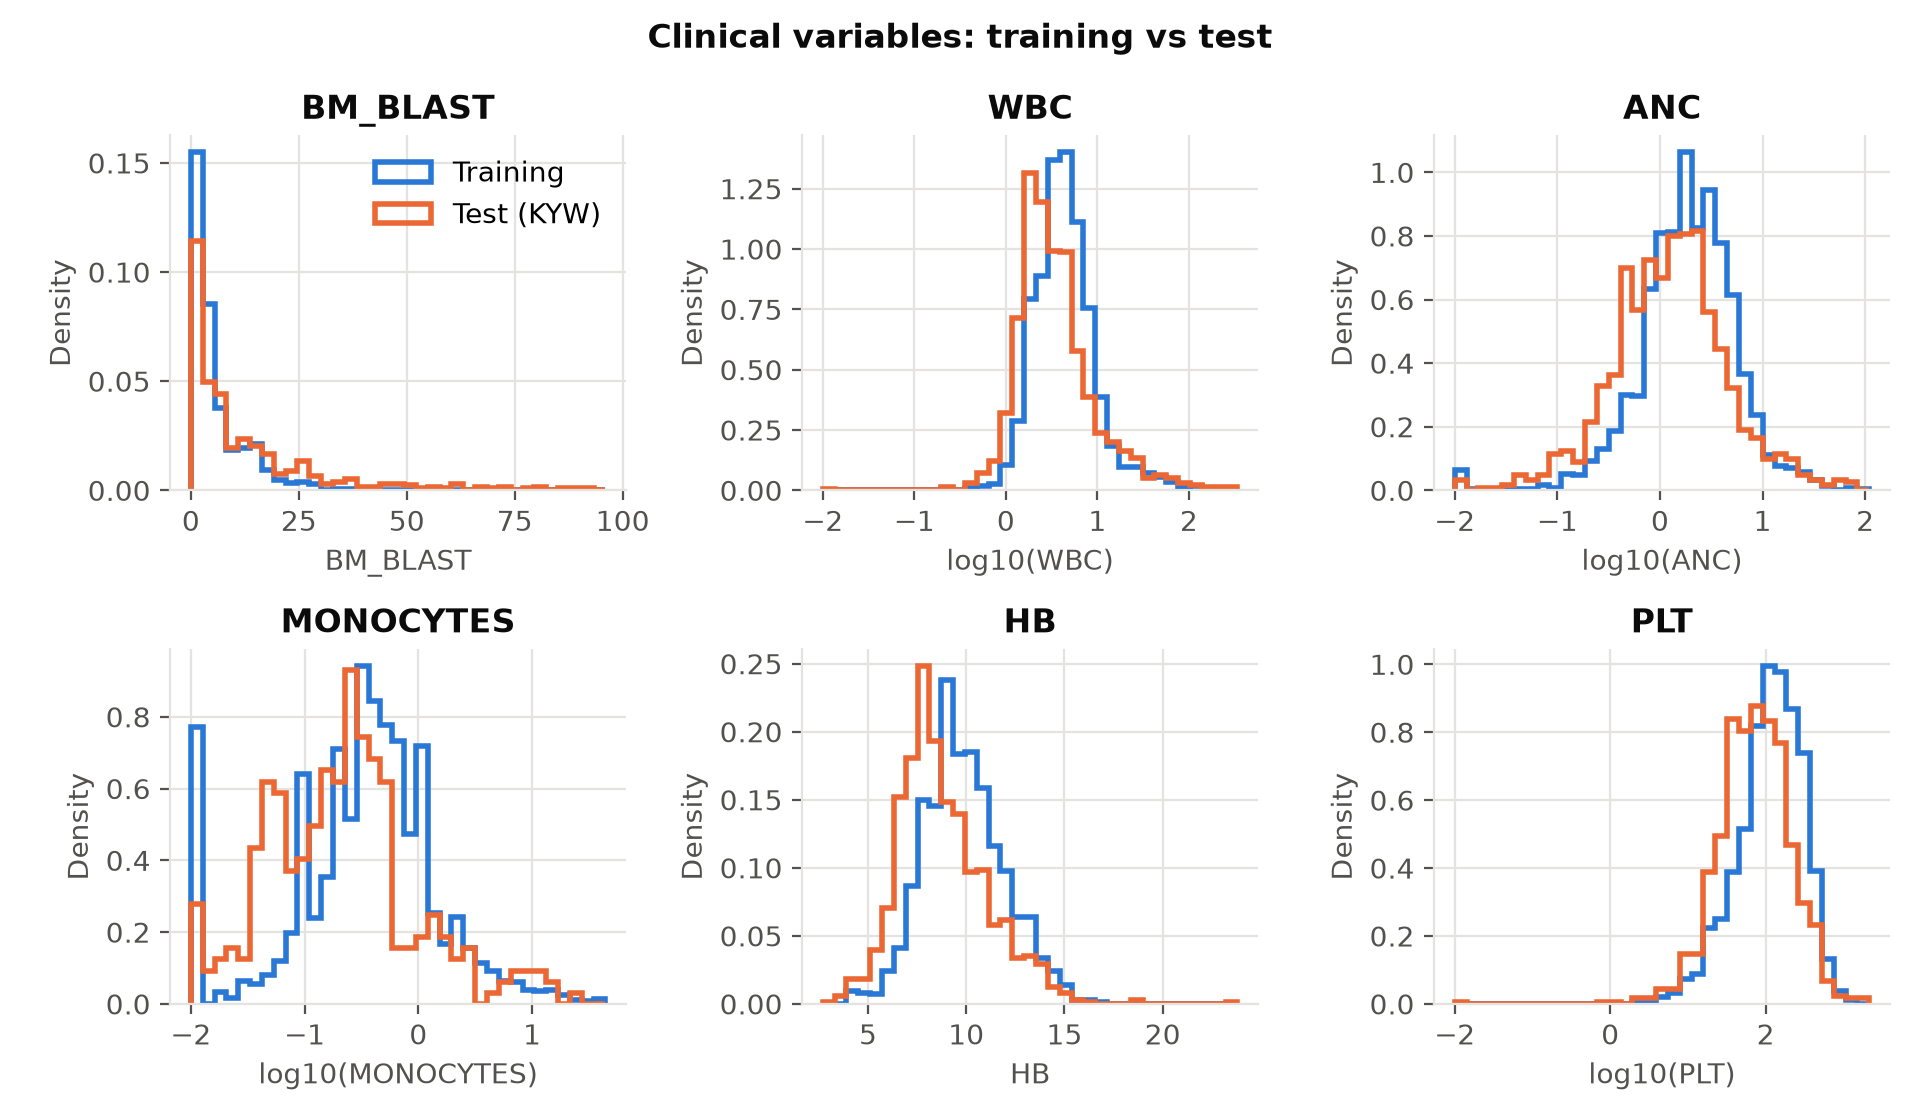
\includegraphics[width=\textwidth]{fig02_clinical_distributions.png}
\caption{Distributions of the clinical variables in training (blue) and test (orange).
Each histogram is scaled to area one so that sets of different sizes can be compared.
Skewed blood counts are shown on a $\log_{10}$ scale; the spike at $-2$ for monocytes
corresponds to recorded values of zero.}
\label{fig:dist}
\end{figure}

The test patients are clinically sicker: lower haemoglobin and platelets, lower
neutrophils, and a much larger share with bone-marrow blasts above 20\%
(17.6\% versus 4.2\%). Monocytes are missing for 74\% of test patients (883 of 1{,}193),
so a model that leans on that variable would be fragile on the test set: all 883 would
receive the same imputed value, and the training median (0.37) is above the test
centre's own median (0.20).

\subsection{Gene mutations}
Training patients carry on average 3.29 recorded mutations and test patients 2.59;
297 training and 139 test patients have none, which is genuine information rather than
missing data. Training data contain 124 distinct genes and test data 83, of which 19
never appear in training. Of the training rows, 114 lack a chromosomal position: they
are partial tandem duplications of \textit{MLL} (89) and internal tandem duplications
of \textit{FLT3} (25), which are structural events rather than single-base changes.
In 1{,}274 cases the same gene is mutated more than once in one patient.

\begin{table}[H]
\centering
\caption{Ten most frequently mutated genes in training: percentage of patients with at
least one mutation.}
\label{tab:genes}
\begin{tabular}{lrr}
\toprule
Gene & Train (\%) & Test (\%) \\
\midrule
\textit{TET2}   & 31.1 & 17.5 \\
\textit{ASXL1}  & 26.9 & 12.7 \\
\textit{SF3B1}  & 22.2 & 7.7 \\
\textit{SRSF2}  & 17.2 & 9.1 \\
\textit{DNMT3A} & 16.1 & 11.1 \\
\textit{RUNX1}  & 13.9 & 13.7 \\
\textit{TP53}   & 11.4 & 25.7 \\
\textit{STAG2}  & 9.1  & 6.7 \\
\textit{U2AF1}  & 8.6  & 8.4 \\
\textit{EZH2}   & 6.5  & 6.7 \\
\bottomrule
\end{tabular}
\end{table}

\begin{figure}[H]
\centering
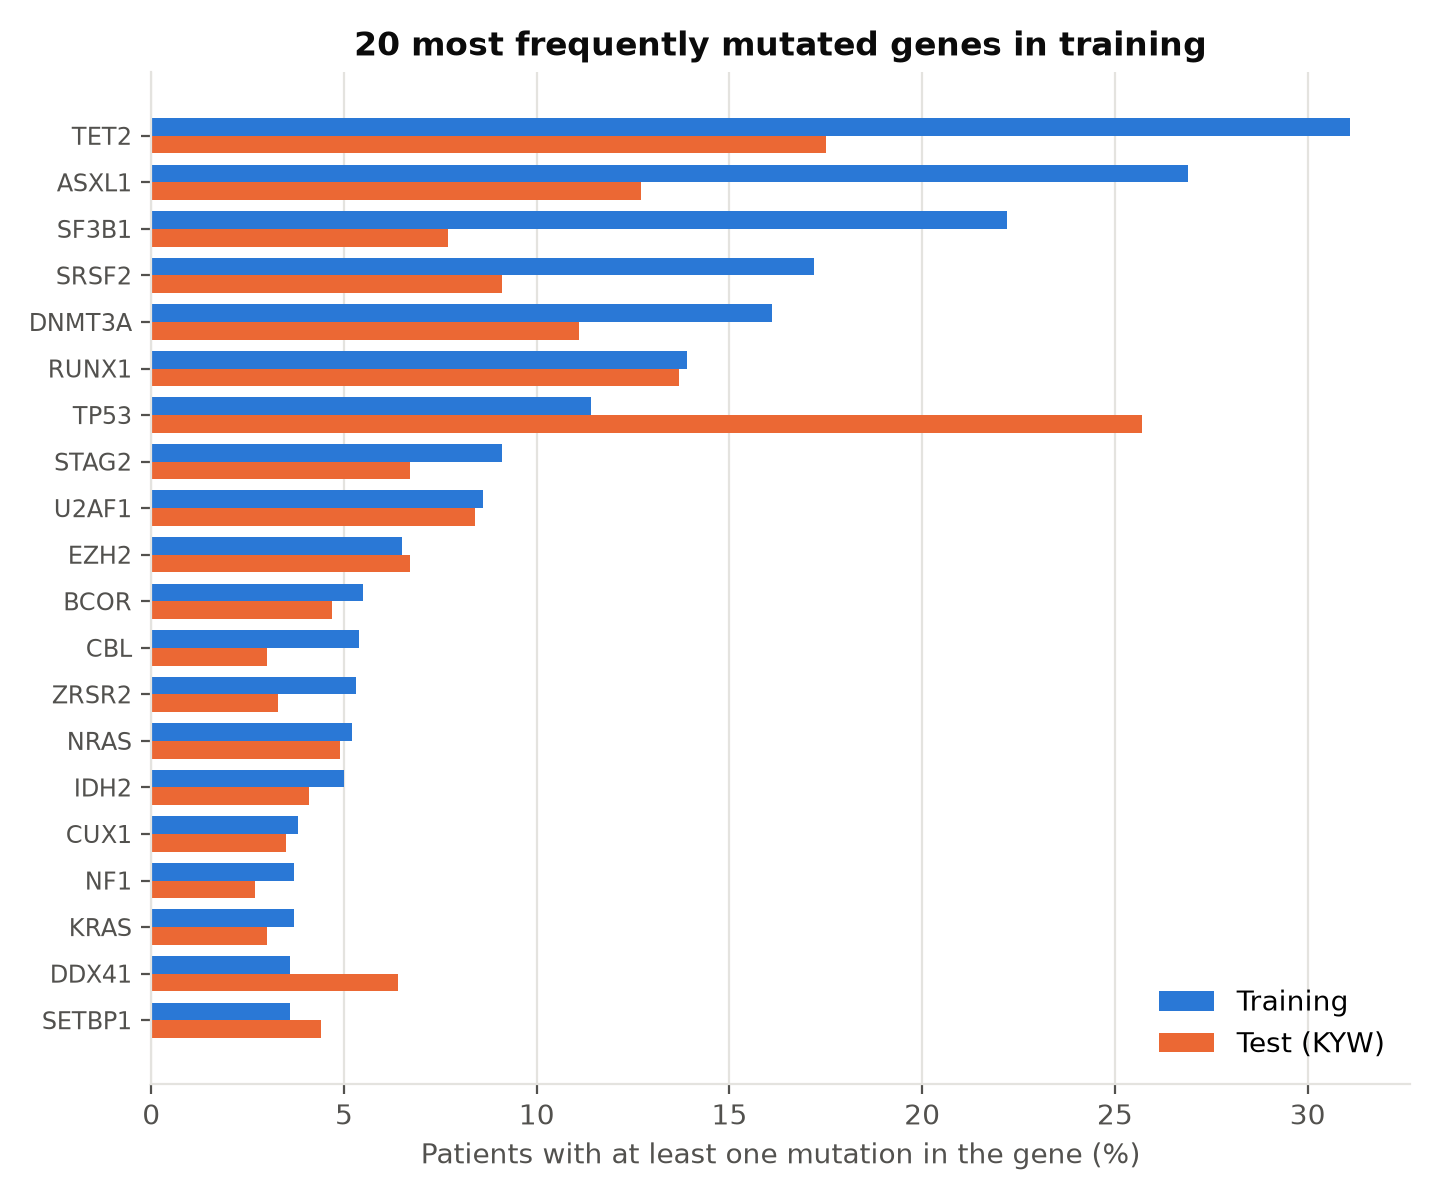
\includegraphics[width=0.8\textwidth]{fig05_gene_frequencies.png}
\caption{The twenty most frequently mutated genes in training, with their frequency in
the test centre.}
\label{fig:genes}
\end{figure}

The most striking difference is \textit{TP53}, mutated in 25.7\% of test patients
against 11.4\% in training (Table~\ref{tab:genes}, Figure~\ref{fig:genes}).
\textit{TP53} mutations are associated with poor prognosis in myeloid neoplasms, which
is consistent with the sicker clinical profile of the test centre. By contrast,
\textit{SF3B1} mutations, typically associated with lower-risk disease, are almost three
times rarer in the test set.

\subsection{Cytogenetics text}
In training, karyotypes are written in lower case (\texttt{46,xy}); in the test set
they are written in upper case (\texttt{46,XY}), and 241 test patients have the single
word \texttt{Normal}. Any parsing must first convert text to lower case and map
\texttt{Normal} to a normal karyotype; otherwise every test karyotype would look
unfamiliar to the model.

\subsection{Consequences for modelling}
\begin{enumerate}
  \item Exclude the 150 training patients without outcome.
  \item Validate with cross-validation grouped by centre, and do not use
        \texttt{CENTER} as a predictor.
  \item Prefer features that are measured consistently in both sets; treat
        \texttt{MONOCYTES} with caution.
  \item Normalise the cytogenetics text before extracting features.
  \item Encode ``no mutation found'' as zero, not as missing.
\end{enumerate}

% ==================================================================
\section{Survival analysis without a model (Stage 2)}
% ==================================================================

\subsection{The Kaplan--Meier estimator}
Let $t_1 < t_2 < \dots$ be the distinct times at which at least one death occurs. At
each $t_k$ let $n_k$ be the number of patients still \emph{at risk} just before $t_k$
(neither dead nor censored yet) and $d_k$ the number of deaths at $t_k$. The
Kaplan--Meier estimator~\cite{kaplan1958} of the survival function is
\begin{equation}
\hat S(t) = \prod_{k:\ t_k \le t} \left(1 - \frac{d_k}{n_k}\right).
\label{eq:km}
\end{equation}
In plain language: to survive past $t_k$ you must survive every earlier death time,
and at each one the chance of surviving, given you were still alive, is the share of
the at-risk patients who did not die. Censored patients never make the curve drop;
they simply leave the risk set, so they count fully for as long as they were observed.

Table~\ref{tab:kmsteps} shows the first six steps. The first death occurs on day one
($t = 0.00274$ years) with $n = 3{,}120$ patients at risk: this is $3{,}173 - 53$, because
the 53 patients with an observed time of zero were all censored at that time and left
the risk set immediately. The first two steps are
\begin{align*}
\hat S(0.00274) &= 1 - \tfrac{1}{3120} = 0.99968,\\
\hat S(0.00822) &= 0.99968 \times \left(1 - \tfrac{2}{3114}\right)
                 = 0.99968 \times 0.99936 = 0.99904.
\end{align*}
My hand implementation of Equation~\eqref{eq:km} agrees with the \texttt{lifelines}
library~\cite{lifelines2019} at every death time to within $2\times 10^{-14}$.

\begin{table}[H]
\centering
\caption{First six steps of the Kaplan--Meier estimator, computed by hand.}
\label{tab:kmsteps}
\begin{tabular}{rrrrr}
\toprule
$t_k$ (years) & $n_k$ & $d_k$ & $1 - d_k/n_k$ & $\hat S(t_k)$ \\
\midrule
0.00274 & 3120 & 1 & 0.99968 & 0.99968 \\
0.00822 & 3114 & 2 & 0.99936 & 0.99904 \\
0.01644 & 3107 & 1 & 0.99968 & 0.99872 \\
0.02192 & 3103 & 2 & 0.99936 & 0.99807 \\
0.02466 & 3098 & 1 & 0.99968 & 0.99775 \\
0.02740 & 3095 & 2 & 0.99935 & 0.99711 \\
\bottomrule
\end{tabular}
\end{table}

The median overall survival, the first time at which $\hat S(t) \le 0.5$, is
\textbf{3.15 years}. Table~\ref{tab:kmyears} and Figure~\ref{fig:kmoverall} give the
whole curve.

\begin{table}[H]
\centering
\caption{Kaplan--Meier overall survival with 95\% confidence intervals.}
\label{tab:kmyears}
\begin{tabular}{rrr}
\toprule
Years & $\hat S(t)$ & 95\% CI \\
\midrule
1 & 0.790 & 0.774--0.804 \\
2 & 0.614 & 0.595--0.633 \\
3 & 0.509 & 0.489--0.529 \\
5 & 0.364 & 0.342--0.386 \\
7 & 0.275 & 0.250--0.299 \\
\bottomrule
\end{tabular}
\end{table}

\begin{figure}[H]
\centering
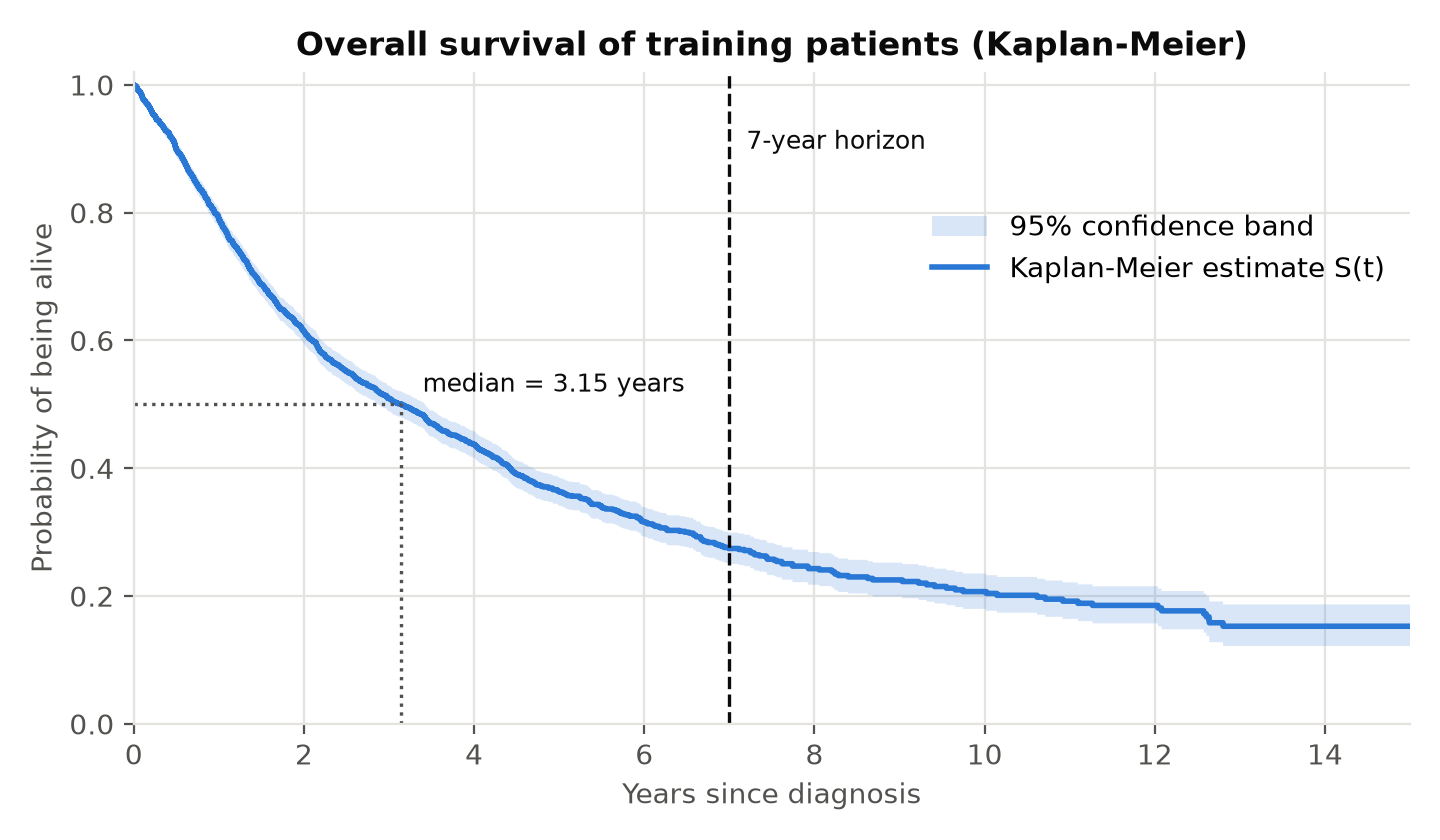
\includegraphics[width=0.9\textwidth]{fig06_km_overall.png}
\caption{Kaplan--Meier estimate of overall survival for the 3{,}173 training patients,
with a 95\% confidence band.}
\label{fig:kmoverall}
\end{figure}

\subsection{Comparing groups: the log-rank test}
To ask whether two groups have different survival, the log-rank
test~\cite{mantel1966} compares, at each death time, the deaths observed in group~1
with the deaths it would receive if the groups were identical. With $n$ at risk in
total, $n_1$ in group~1, $n_2 = n - n_1$, $d$ deaths in total and $d_1$ in group~1,
\begin{equation}
E_{1k} = d\,\frac{n_1}{n}, \qquad
V_k = \frac{n_1\, n_2\, d\,(n - d)}{n^2 (n-1)}, \qquad
\chi^2 = \frac{\left(\sum_k (d_{1k} - E_{1k})\right)^2}{\sum_k V_k},
\label{eq:logrank}
\end{equation}
which follows a $\chi^2$ distribution with one degree of freedom when the groups do not
differ. In plain language: group~1 should get ``its fair share'' $n_1/n$ of the deaths
at each time; $\chi^2$ measures how far the total gap is from zero, in units of its own
variability.

\paragraph{Worked example: \textit{TP53}.}
Summing over all death times, the 368 patients with a \textit{TP53} mutation had
$O_1 = 271$ observed deaths against $E_1 = 112.13$ expected, with total variance
$V = 103.17$. Hence
\[
\chi^2 = \frac{(271 - 112.13)^2}{103.17} = \frac{158.87^2}{103.17} = 244.64,
\qquad p = 3.8\times 10^{-55},
\]
identical to the \texttt{lifelines} result. \textit{TP53}-mutated patients died more
than twice as often as expected under ``no difference''.

Table~\ref{tab:logrank} and Figure~\ref{fig:kmgroups} show four comparisons. Monosomy~7
was detected in the karyotype text as ``\texttt{-7}'' after a comma, slash or the
start of the string and not followed by another digit; 79 patients without a blast
value are left out of the blast comparison.

\begin{table}[H]
\centering
\caption{Kaplan--Meier summaries and log-rank tests by group. All $p < 0.001$.}
\label{tab:logrank}
\begin{tabular}{llrrrrr}
\toprule
Comparison & Group & $n$ & Deaths & Median (y) & $\hat S(3)$ & $\chi^2$ (df) \\
\midrule
Blasts & $<5\%$      & 2015 & 841  & 4.47 & 0.620 & \multirow{3}{*}{272.1 (2)} \\
       & 5--20\%     & 942  & 622  & 1.68 & 0.326 & \\
       & $>20\%$     & 137  & 89   & 1.19 & 0.238 & \\
\midrule
\textit{TP53}  & not mutated & 2805 & 1329 & 3.59 & 0.549 & \multirow{2}{*}{244.6 (1)} \\
               & mutated     & 368  & 271  & 1.00 & 0.207 & \\
\midrule
Monosomy 7     & no          & 3008 & 1477 & 3.41 & 0.528 & \multirow{2}{*}{139.5 (1)} \\
               & yes         & 165  & 123  & 0.95 & 0.169 & \\
\midrule
\textit{SF3B1} & not mutated & 2446 & 1289 & 2.57 & 0.463 & \multirow{2}{*}{51.8 (1)} \\
               & mutated     & 727  & 311  & 4.56 & 0.665 & \\
\bottomrule
\end{tabular}
\end{table}

\begin{figure}[H]
\centering
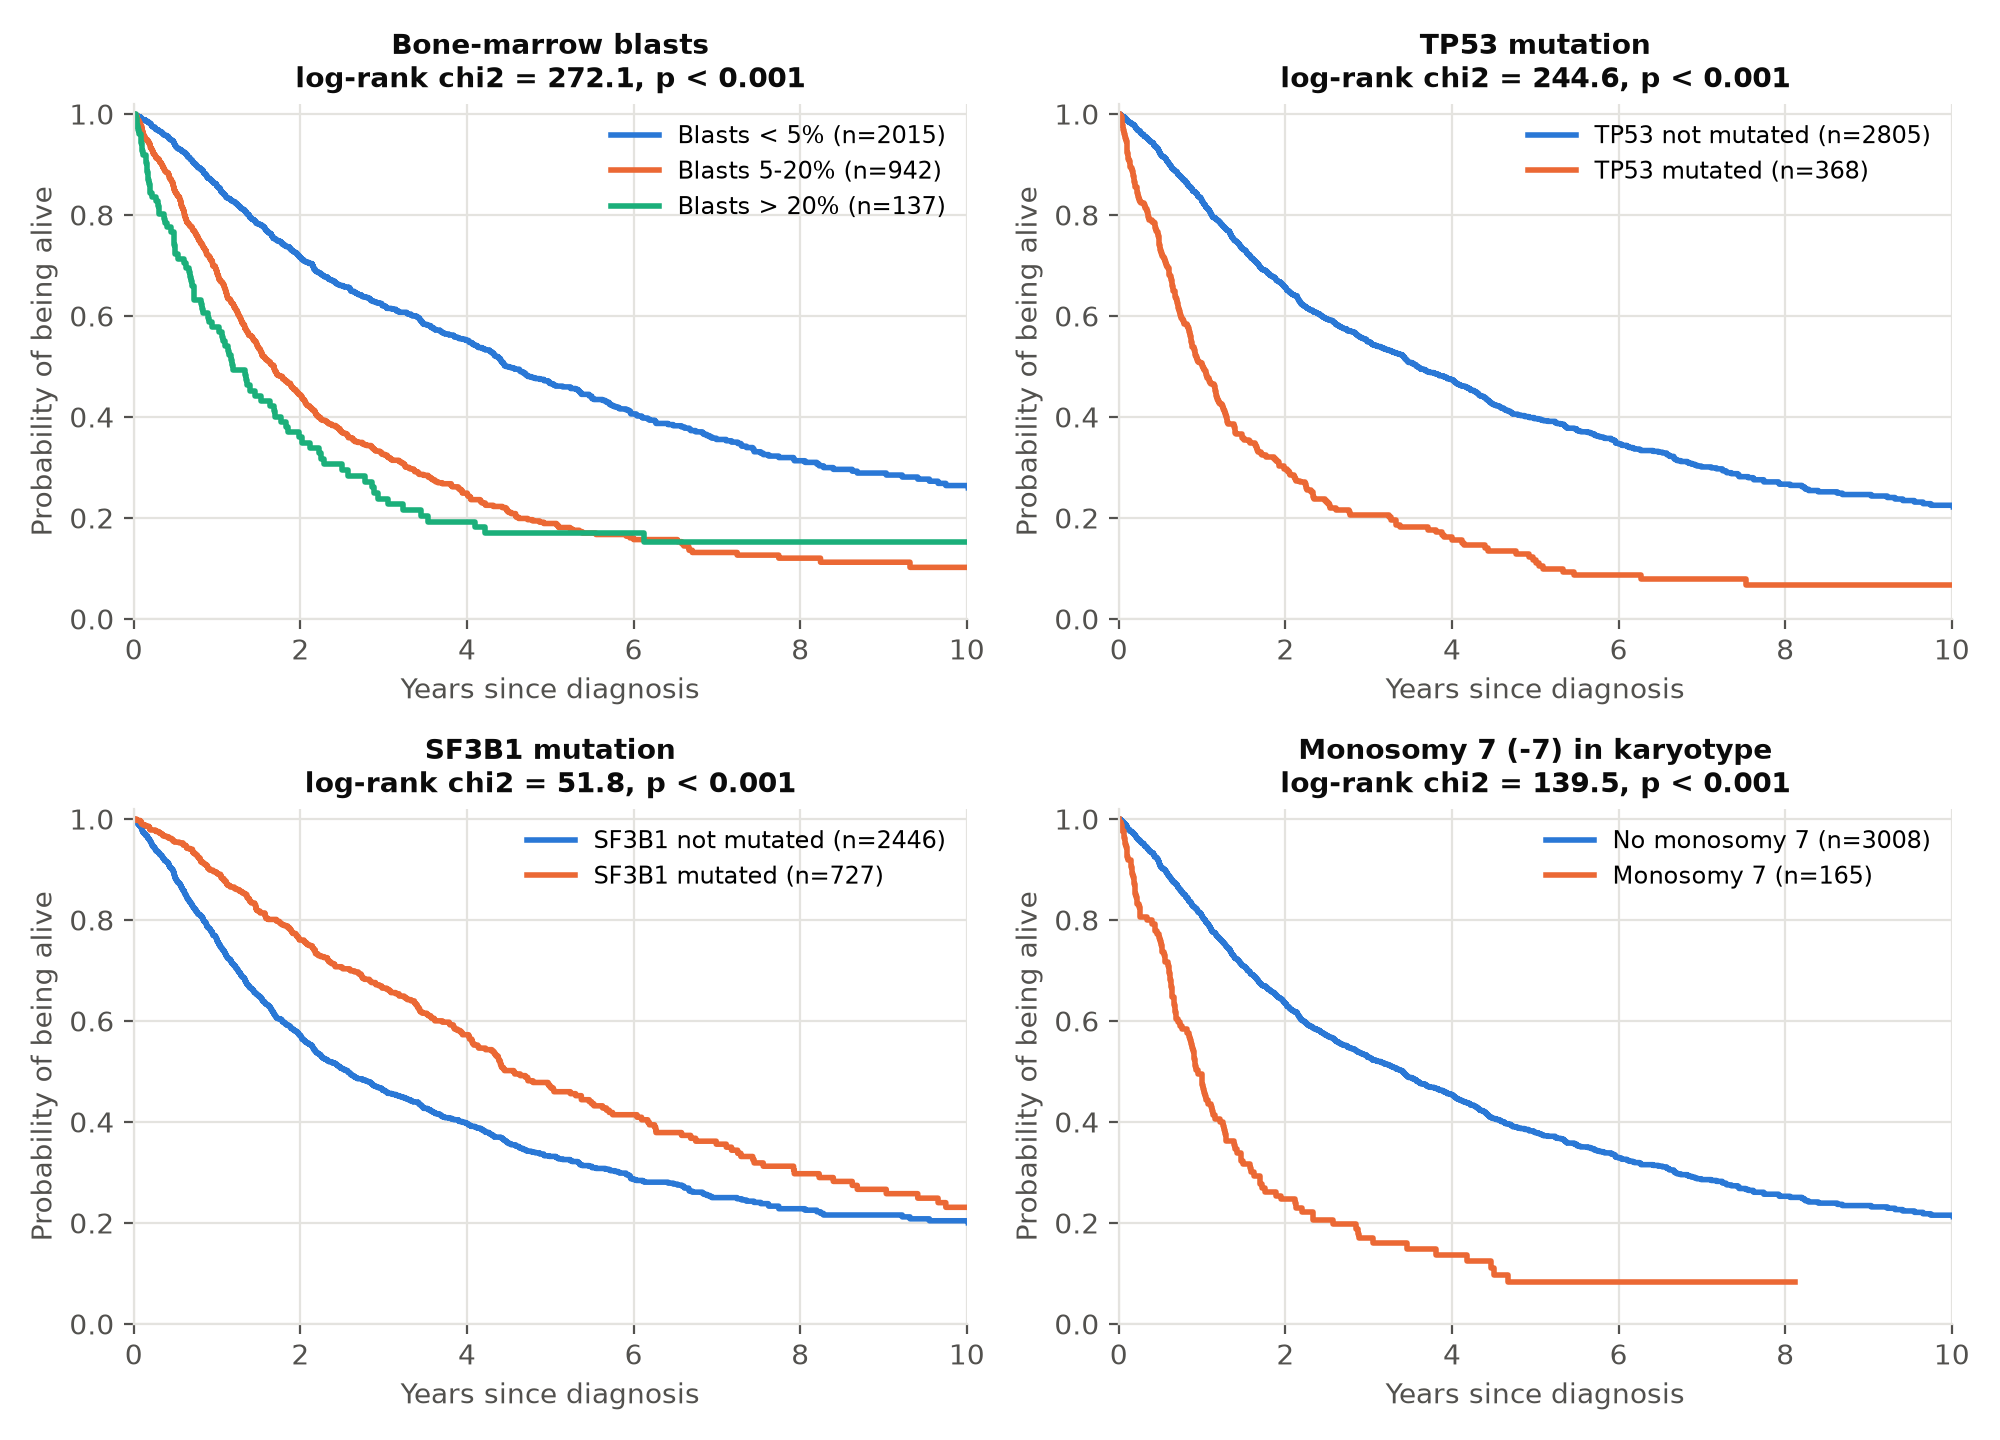
\includegraphics[width=\textwidth]{fig07_km_groups.png}
\caption{Kaplan--Meier curves by bone-marrow blast level, \textit{TP53} mutation,
\textit{SF3B1} mutation and monosomy~7.}
\label{fig:kmgroups}
\end{figure}

Higher blasts, \textit{TP53} mutation and monosomy~7 all shorten survival sharply; the
median survival of \textit{TP53}-mutated patients is one year against 3.59 years for the
rest. \textit{SF3B1} is protective: mutated patients have a median survival of 4.56
years against 2.57. These directions agree with established clinical risk
stratification and with the sicker profile of the test centre noted in Stage~1.

\subsection{The censoring curve}
Swapping the roles of death and censoring in Equation~\eqref{eq:km}, so that the
``event'' is being censored, gives the \emph{reverse Kaplan--Meier} estimate
$\hat G(t)$: the probability that a patient is still being followed at time $t$. This
is exactly the $\hat G$ in the metric (Equation~\eqref{eq:uno}).

\begin{table}[H]
\centering
\caption{Censoring curve and the resulting metric weight of a death at time $t$.}
\label{tab:gcurve}
\begin{tabular}{rrr}
\toprule
$t$ (years) & $\hat G(t)$ & weight $1/\hat G(t)^2$ \\
\midrule
1 & 0.827 & $1/0.827^2 = 1.46$ \\
3 & 0.613 & $1/0.613^2 = 2.66$ \\
5 & 0.347 & $1/0.347^2 = 8.32$ \\
7 & 0.198 & $1/0.198^2 = 25.61$ \\
\bottomrule
\end{tabular}
\end{table}

\begin{figure}[H]
\centering
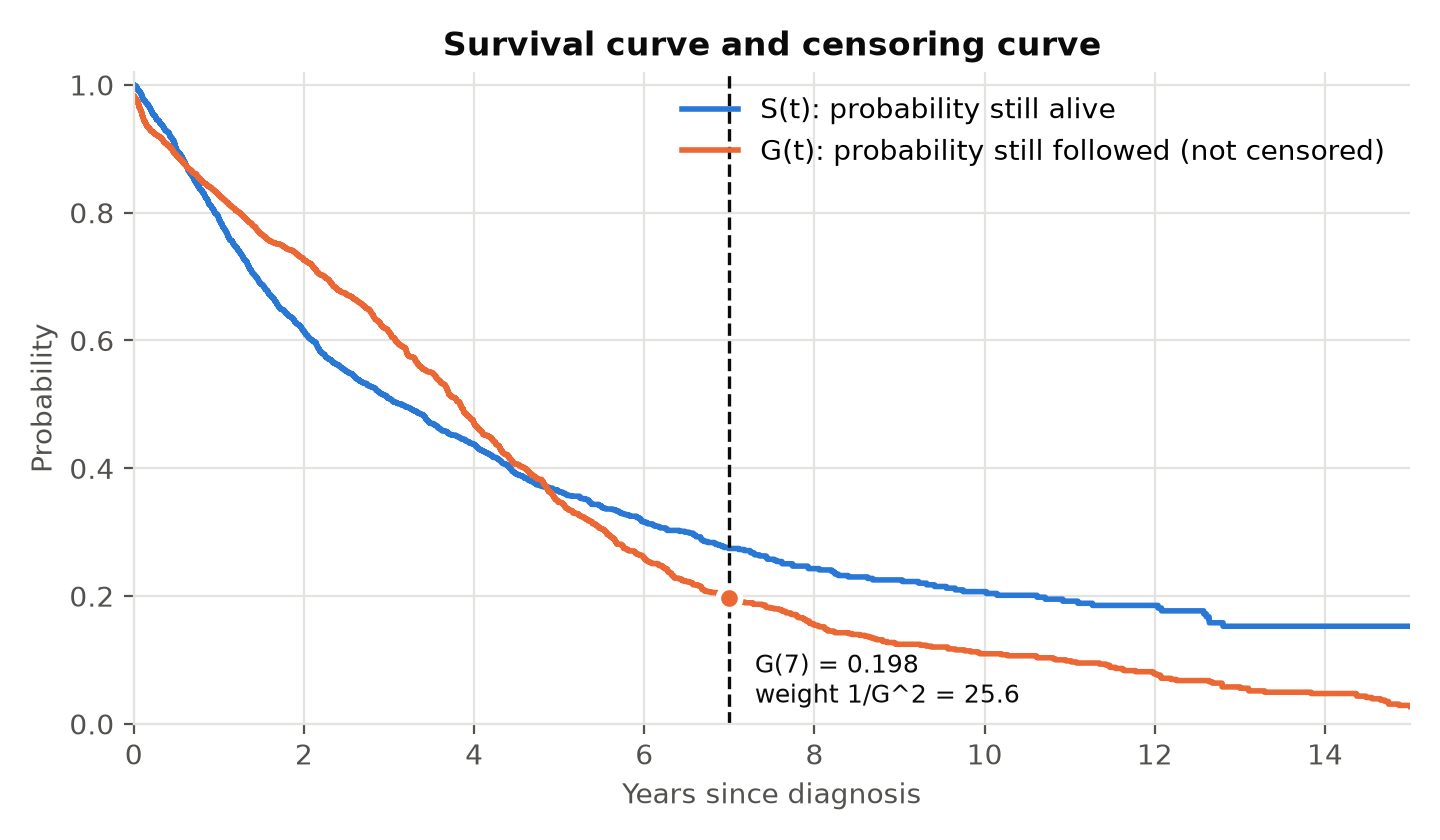
\includegraphics[width=0.9\textwidth]{fig08_censoring_curve.png}
\caption{Survival curve $\hat S(t)$ and censoring curve $\hat G(t)$. By seven years only
19.8\% of patients are still being followed.}
\label{fig:gcurve}
\end{figure}

Table~\ref{tab:gcurve} shows the practical effect: a pair started by a death just
before seven years weighs about $25.6/1.46 \approx 17.5$ times as much as one started
by a death at one year. A model that ranks late deaths poorly is therefore penalised
far more by the challenge metric than by Harrell's C.

\subsection{The metric by hand: a six-patient example}
Figure~\ref{fig:toy} shows six patients with observed times, statuses and risk scores.

\begin{figure}[H]
\centering
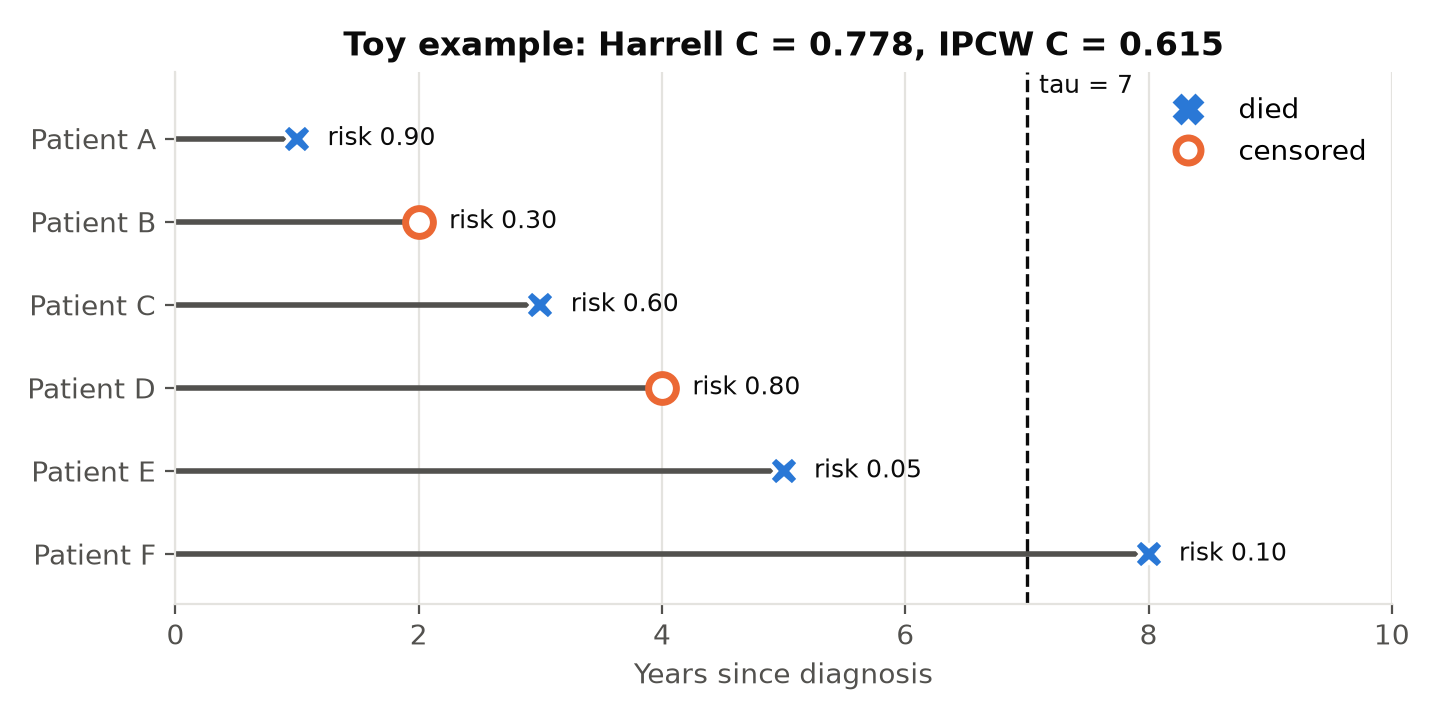
\includegraphics[width=0.9\textwidth]{fig09_toy_example.png}
\caption{Toy example: crosses are deaths, circles are censored patients; each patient
carries a risk score.}
\label{fig:toy}
\end{figure}

\paragraph{Comparable pairs.} Only deaths can start a comparable pair, and only with
patients observed for longer. Patient~A (death at 1) is comparable with B, C, D, E, F;
patient~C (death at 3) with D, E, F; patient~E (death at 5) with F; patient~F (death at
8) has nobody after it. That gives $5 + 3 + 1 = 9$ comparable pairs. Of these, two are
discordant: $(C, D)$ because $0.60 < 0.80$ and $(E, F)$ because $0.05 < 0.10$. So
\[
C_{\text{Harrell}} = \frac{7}{9} = 0.778.
\]

\paragraph{Censoring curve.} Censorings occur at $t=2$ (B), with 5 patients at risk,
and at $t = 4$ (D), with 3 at risk:
\[
\hat G(2) = 1 - \tfrac{1}{5} = 0.8, \qquad
\hat G(4) = 0.8 \times \left(1 - \tfrac{1}{3}\right) = 0.5333.
\]
So $\hat G(1) = 1$, $\hat G(3) = 0.8$ and $\hat G(5) = 0.5333$, giving the weights
\[
w_A = \frac{1}{1^2} = 1, \qquad
w_C = \frac{1}{0.8^2} = 1.5625, \qquad
w_E = \frac{1}{0.5333^2} = 3.5156.
\]
Patient F died at $8 \ge \tau = 7$ and starts no pair anyway.

\paragraph{IPCW C-index.}
\begin{align*}
\text{numerator}   &= 5\times 1 + 2 \times 1.5625 + 0 \times 3.5156 = 8.1250,\\
\text{denominator} &= 5\times 1 + 3 \times 1.5625 + 1 \times 3.5156 = 13.2031,\\
C_7 &= \frac{8.1250}{13.2031} = 0.615.
\end{align*}
Both values match \texttt{scikit-survival} exactly. The IPCW value is lower because both
wrong pairs start from later deaths (C at 3 years, E at 5 years), whose weights are
larger.

\subsection{Single-variable baselines}
Before fitting any model, each variable can be used directly as a risk score, with its
direction fixed by clinical knowledge rather than learned from the outcome (missing
values set to the median). Table~\ref{tab:single} and Figure~\ref{fig:single} give the
results on the 3{,}173 training patients.

\begin{table}[H]
\centering
\caption{Concordance of single-variable risk scores ($\tau = 7$ years).}
\label{tab:single}
\begin{tabular}{lrr}
\toprule
Risk score & Harrell's C & IPCW C \\
\midrule
Random numbers (reference)      & 0.509 & 0.509 \\
$+$ bone-marrow blasts          & 0.631 & 0.616 \\
$-$ platelets                   & 0.631 & 0.608 \\
$+$ number of mutations         & 0.602 & 0.605 \\
$-$ haemoglobin                 & 0.603 & 0.593 \\
$+$ \textit{TP53} mutated (0/1) & 0.566 & 0.553 \\
$-$ \textit{SF3B1} mutated (0/1)& 0.554 & 0.544 \\
$+$ monosomy 7 (0/1)            & 0.532 & 0.526 \\
$-$ bone-marrow blasts (wrong sign) & 0.369 & 0.384 \\
\bottomrule
\end{tabular}
\end{table}

\begin{figure}[H]
\centering
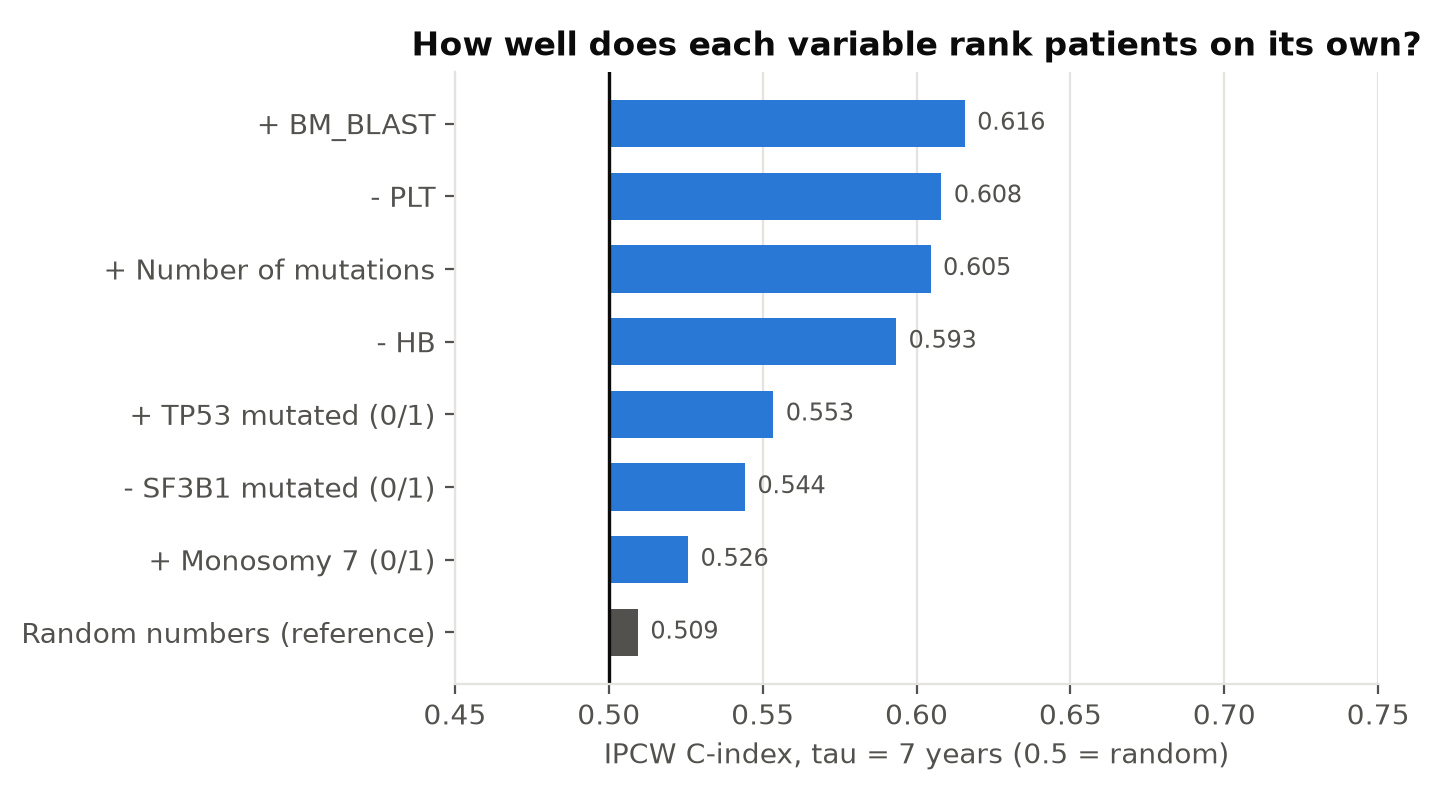
\includegraphics[width=0.85\textwidth]{fig10_single_variable_cindex.png}
\caption{IPCW C-index of each single-variable risk score; 0.5 corresponds to random
ranking.}
\label{fig:single}
\end{figure}

Three lessons follow. First, reversing the sign of a score turns $C$ into $1 - C$
($0.631 \to 0.369$), so the direction of a risk score matters. Second, binary markers
rank poorly on their own even when their log-rank test is overwhelming:
\textit{TP53} has $\chi^2 = 244.6$ but an IPCW C of only 0.553. Only 11.6\% of patients
carry the mutation, so most comparable pairs have equal scores and count one half.
Statistical significance and ranking power are different things. Third, no single
variable exceeds about 0.62, so combining them in a multivariable model is necessary.

% ==================================================================
\section{Next steps}
% ==================================================================
Stage 3 will build features: clinical transforms and missing-value handling,
cytogenetic indicators parsed from the normalised karyotype text (normal karyotype,
monosomy~7, deletion 5q, complex karyotype and others), and mutation features (gene
indicators, number of mutations, maximum VAF). All steps that learn from data will be
fitted inside cross-validation folds. Stage 4 will then fit Cox models under
centre-grouped cross-validation and produce the first submission.

% ==================================================================
\begin{thebibliography}{9}

\bibitem{noren2016}
D.~P. Noren \textit{et al.},
A crowdsourcing approach to developing and assessing prediction algorithms for AML
prognosis,
\textit{PLOS Computational Biology}, 12(6): e1004890, 2016.

\bibitem{harrell1982}
F.~E. Harrell, R.~M. Califf, D.~B. Pryor, K.~L. Lee and R.~A. Rosati,
Evaluating the yield of medical tests,
\textit{JAMA}, 247(18): 2543--2546, 1982.

\bibitem{uno2011}
H.~Uno, T.~Cai, M.~J. Pencina, R.~B. D'Agostino and L.~J. Wei,
On the C-statistics for evaluating overall adequacy of risk prediction procedures
with censored survival data,
\textit{Statistics in Medicine}, 30(10): 1105--1117, 2011.

\bibitem{polsterl2020}
S.~P\"olsterl,
scikit-survival: a library for time-to-event analysis built on top of scikit-learn,
\textit{Journal of Machine Learning Research}, 21(212): 1--6, 2020.

\bibitem{kaplan1958}
E.~L. Kaplan and P.~Meier,
Nonparametric estimation from incomplete observations,
\textit{Journal of the American Statistical Association}, 53(282): 457--481, 1958.

\bibitem{mantel1966}
N.~Mantel,
Evaluation of survival data and two new rank order statistics arising in its
consideration,
\textit{Cancer Chemotherapy Reports}, 50(3): 163--170, 1966.

\bibitem{lifelines2019}
C.~Davidson-Pilon,
lifelines: survival analysis in Python,
\textit{Journal of Open Source Software}, 4(40): 1317, 2019.

\end{thebibliography}

\end{document}
